%%%%%%%%%%%%%%%%%%%%%%%%%%%%%%%%%%%%%%%%%%%%%%%%%%%%%%%%%%%%%%%%%%%%%%%%%%%%
%% Author template for Interfaces (inte)
%% Mirko Janc, Ph.D., INFORMS, mirko.janc@informs.org
%% ver. 0.95, December 2010
%%%%%%%%%%%%%%%%%%%%%%%%%%%%%%%%%%%%%%%%%%%%%%%%%%%%%%%%%%%%%%%%%%%%%%%%%%%%
\documentclass[inte,blindrev]{informs3}
%\documentclass[inte,nonblindrev]{informs3} % current default for manuscript submission

%%\OneAndAHalfSpacedXI
%\OneAndAHalfSpacedXII % Current default line spacing
%\DoubleSpacedXII
\DoubleSpacedXI

% If hyperref is used, dvi-to-ps driver of choice must be declared as
%   an additional option to the \documentclass. For example
%\documentclass[dvips,inte]{informs3}      % if dvips is used
%\documentclass[dvipsone,inte]{informs3}   % if dvipsone is used, etc.

% Private macros here (check that there is no clash with the style)

% Natbib setup for author-year style
\usepackage{natbib}
 \bibpunct[, ]{(}{)}{,}{a}{}{,}%
 \def\bibfont{\small}%
 \def\bibsep{\smallskipamount}%
 \def\bibhang{24pt}%
 \def\newblock{\ }%
 \def\BIBand{and}%

%% Setup of theorem styles. Outcomment only one. 
%% Preferred default is the first option.
\TheoremsNumberedThrough     % Preferred (Theorem 1, Lemma 1, Theorem 2)
%\TheoremsNumberedByChapter  % (Theorem 1.1, Lema 1.1, Theorem 1.2)

%% Setup of the equation numbering system. Outcomment only one.
%% Preferred default is the first option.
\EquationsNumberedThrough    % Default: (1), (2), ...
%\EquationsNumberedBySection % (1.1), (1.2), ...

% In the reviewing and copyediting stage enter the manuscript number.
%\MANUSCRIPTNO{} % When the article is logged in and DOI assigned to it,
                 %   this manuscript number is no longer necessary

\setcounter{secnumdepth}{0}% "Interfaces" does not number sections

%%%%%%%%%%%%%%%%
\begin{document}
%%%%%%%%%%%%%%%%

% Outcomment only when entries are known. Otherwise leave as is and 
%   default values will be used.
%\setcounter{page}{1}
%\VOLUME{00}%
%\NO{0}%
%\MONTH{Xxxxx}% (month or a similar seasonal id)
%\YEAR{0000}% e.g., 2005
%\FIRSTPAGE{000}%
%\LASTPAGE{000}%
%\SHORTYEAR{00}% shortened year (two-digit)
%\ISSUE{0000} %
%\LONGFIRSTPAGE{0001} %
%\DOI{10.1287/xxxx.0000.0000}%

% Author's names for the running heads
% Sample depending on the number of authors;
\RUNAUTHOR{Duan}
% \RUNAUTHOR{Jones and Wilson}
% \RUNAUTHOR{Jones, Miller, and Wilson}
% \RUNAUTHOR{Jones et al.} % for four or more authors
% Enter authors following the given pattern:
%\RUNAUTHOR{}

% Title or shortened title suitable for running heads. Sample:
\RUNTITLE{Home Field Advantage in Professional Soccer Competition}
% Enter the (shortened) title:
%\RUNTITLE{}

% Full title. Sample:
\TITLE{Home Sweet Home Field Advantage: An Bayesian Analysis at the Season Level}
% Enter the full title:
%\TITLE{}

% Block of authors and their affiliations starts here:
% NOTE: Authors with same affiliation, if the order of authors allows, 
%   should be entered in ONE field, separated by a comma. 
%   \EMAIL field can be repeated if more than one author
\ARTICLEAUTHORS{%
\AUTHOR{C.J. (Chaojie) Duan}
\AFF{Troy University, \EMAIL{cjduan@outlook.com}}
\AUTHOR{Ananyo Chakravarty}
\AFF{Troy University, \EMAIL{achakravarty@troy.edu}}
% Enter all authors
} % end of the block

\ABSTRACT{%
Using  season-long performance data  collected from the ESPN FC website.% Enter your abstract
}%

% Sample 
%\KEYWORDS{deterministic inventory theory; infinite linear programming duality; 
%  existence of optimal policies; semi-Markov decision process; cyclic schedule}
%\HISTORY{This article was reviewed} % for example

% Fill in data. If unknown, or unnecessary, outcomment the field
\KEYWORDS{European Professional Soccer Leagues, Home Field Advantage, Bayesian Statistical Inference, Most Home Goals, Most Away Goals}
%\HISTORY{}

\maketitle
%%%%%%%%%%%%%%%%%%%%%%%%%%%%%%%%%%%%%%%%%%%%%%%%%%%%%%%%%%%%%%%%%%%%%%

% Samples of sectioning (and labeling) in INTE
% NOTE: (1) \section and \subsection do NOT end with a period
%       (2) \subsubsection and lower need end punctuation
%       (3) capitalization is as shown (title style).
%
%\section{Introduction.}\label{intro} %%1.
%\subsection{Duality and the Classical EOQ Problem.}\label{class-EOQ} %% 1.1.
%\subsection{Outline.}\label{outline1} %% 1.2.
%\subsubsection{Cyclic Schedules for the General Deterministic SMDP.}
%  \label{cyclic-schedules} %% 1.2.1
%\section{Problem Description.}\label{problemdescription} %% 2.

% Text of your paper here

\section{Introduction}

The popular frequentist statistical inference process starts with the formulation of an alternative research hypothesis(Ha), such as "people with higher income live happier than low income earners", which is typically set up against a null non-effect hypothesis (Ho), such as ``income level has no effect on happiness". Then researchers collect relevant data (each subject's perceived happiness and income), and conduct a statistical  
\citep{Tipping2004bayesian}
\section*{Context and Data}

According to ESPN FC(www.espnfc.us), eight season-long performance metrics are used to characterize a professional soccer team's regular league season. Below, we define those statistics using the 2015/16 La Liga season of Real Madrid C.F. as an example.
\begin{itemize}
\item Most Home Goals (MHG) = maximum goals scored in a single match played at home. For the season 2015/2016, Real Madrid’s MHG is 10. They beat Rayo Vallecano by 10-2 at Santiago Bernabéu Stadium on 12/20/2015.
\item Most Away Goals (MAG) = maximum goals scored in a single away match. For the season 2015/2016, Real Madrid’s MAG is 6. They defeated Espanyol 6-0 on 9/12/2015 at RCDE stadium.
 
\end{itemize} 
\subsection*{Data Source}
The statistics we use in the present paper are freely available to the public; we develop our own R-based data scraper (program) and use it to extract our data from the website ESPN FC. Our data set covers all of the Big Five (EPL, La Liga, Bundesliga, Leagure 1, Serie A) and spans from seasons 2001/2 - 2015/16. in addition to the eight performance metrics we defined in earlier section, we also collect our response values of aggregated attendance for each team-season unit.   


%===================================================================================
% Acknowledgments here
\ACKNOWLEDGMENT{%
 Enter the text of acknowledgments here
}% Leave this (end of acknowledgment)

%===================================================================================
\bibliographystyle{informs2014} % outcomment this and next line in Case 1
\bibliography{Soccer_Interfaces} % if more than one, comma separated
%==========================================Summary Statistics ====================================
\newpage
\begin{table}
\TABLE {Descriptive Statistics\label{Tab1}}
{\begin{tabular}{|c|c|c|c|c|c|c|}
\hline 
\up\down & Mean & Median & Std. Dev. & Min. & Max. & Interquartile Range \\
\hline 
\up\down MHG & 3.634 & 4 & 1.676 & 0 & 9 & 2\\
\hline 
\up\down MAG & 2.884 & 3 & 1.676 & 0 & 10 & 2\tabularnewline
\hline 
\up\down LMV & 4.319 & 4 & 1.409 & 1 & 10 & 2\tabularnewline
\hline 
LMD & 3.588 & 3 & 1.186 & 1 & 8 & 1\tabularnewline
\hline 
LWS & 4.303 & 4 & 2.254 & 1 & 22 & 2\tabularnewline
\hline 
LUBS & 8.844 & 8 & 5.213 & 2 & 45 & 6\tabularnewline
\hline 
LLS & 2.881 & 3 & 1.283 & 1 & 13 & 2\tabularnewline
\hline 
LDDS & 5.578 & 5 & 2.741 & 1 & 21 & 3\tabularnewline
\hline 
AATT & 705808.736 & 608990.5 & 451624.726 & 4048 & 2477095 & 528828\tabularnewline
\hline 
\end{tabular}}
{all performance variables including attendance}
\end{table}
%============================= Correlation Matrix=================================================
\begin{table}
\TABLE {Correlation Matrix\label{Tab2}}
{\begin{tabular}{|l|r@{\extracolsep{0pt}.}l|r@{\extracolsep{0pt}.}l|r@{\extracolsep{0pt}.}l|r@{\extracolsep{0pt}.}l|r@{\extracolsep{0pt}.}l|r@{\extracolsep{0pt}.}l|r@{\extracolsep{0pt}.}l|r@{\extracolsep{0pt}.}l|r@{\extracolsep{0pt}.}l|}
\hline 
 & \multicolumn{2}{c|}{LLS} & \multicolumn{2}{c|}{LMD} & \multicolumn{2}{c|}{LMV} & \multicolumn{2}{c|}{LUBS} & \multicolumn{2}{c|}{LWLSS} & \multicolumn{2}{c|}{LWS} & \multicolumn{2}{c|}{MAG} & \multicolumn{2}{c|}{MHG} & \multicolumn{2}{c|}{AATT}\tabularnewline
\hline 
LLS & 1&000 & 0&308 & -0&255 & -0&412 & 0&539 & -0&379  & -0&172 & -0&274 & -0&247\tabularnewline
\hline 
LMD & 0&308 & 1&000 & -0&222 & -0&347 & 0&296 & -0&292 & -0&168 & -0&207 & -0&134\tabularnewline
\hline 
LMV & -0&255 & -0&222 & 1&000 & 0&415 & -0&396 & 0&436 & 0&558 & 0&768 & 0&417\tabularnewline
\hline 
LUBS & -0&412 & -0&347 & 0&415 & 1&000 & -0&452 & 0&612 & 0&314 & 0&362 & 0&409\tabularnewline
\hline 
LWLSS & 0&539 & 0&296 & -0&396 & -0&452 & 1&000 & -0&416 & -0&279 & -0&355 & -0&335\tabularnewline
\hline 
LWS & -0&379 & -0&292 & 0&435 & 0&612 & -0&416 & 1&000 & 0&336 & 0&382 & 0&478\tabularnewline
\hline 
MAG & -0&172 & -0&168 & 0&558 & 0&314 & -0&279 & 0&336 & 1&000 & 0&185 & 0&260\tabularnewline
\hline 
MHG & -0&274 & -0&207 & 0&768 & 0&362 & -0&355 & 0&382 & 0&185 & 1&000 & 0&383\tabularnewline
\hline 
AATT & -0&247 & -0&134 & 0&417 & 0&409 & -0&335 & 0&478 & 0&260 & 0&383 & 1&000\tabularnewline
\hline 
\end{tabular}}
{ all coefficients are significant at the p value of 0.001 level}
\end{table}
%==============table of model results ===============
\begin{table}
\TABLE {Model Results\label{Tab3}}
{\begin{tabular}{|l|c|c|c|c|}
\hline 
\multicolumn{1}{|c|}{Variable Name} & \multicolumn{1}{c|}{OLS} & CV-LASSO & CV-Elastic Net & CV-Ridge Regression\tabularnewline
\hline 
MHG & 0.165 ({*}{*}{*}) & 0.149 & 0.152 & 0.159\tabularnewline
\hline 
MAG & 0.029 ({*}{*}{*}) & 0.019 & 0.021 & 0.039\tabularnewline
\hline 
LMV & 0.234 ({*}{*} )  & 0.247 & 0.243 & 0.222\tabularnewline
\hline 
LMD & 0.139 (NS ) & 0.109 & 0.112 & 0.103\tabularnewline
\hline 
LWS & 0.346 ({*}{*}{*}) & 0.341 & 0.339 & 0.294\tabularnewline
\hline 
LUBS & 0.132 ({*}{*}{*}) & 0.125 & 0.127 & 0.131\tabularnewline
\hline 
LLS & 0.004 (NS) &  &  & -0.014\tabularnewline
\hline 
LDDS & -0.114 ({*} )  & -0.105 & -0.106 & -0.106\tabularnewline
\hline 
\multicolumn{1}{|c|}{CV-MSE} & \multicolumn{1}{c|}{0.291} & 0.290 & 0.277 & 0.291\tabularnewline
\hline 
\end{tabular}}
{Tex of notes}
\end{table}


%====================================================
% Acknowledgments here
%\ACKNOWLEDGMENT{%
% Enter the text of acknowledgments here
%}% Leave this (end of acknowledgment)

%========================
\begin{figure}
\FIGURE
{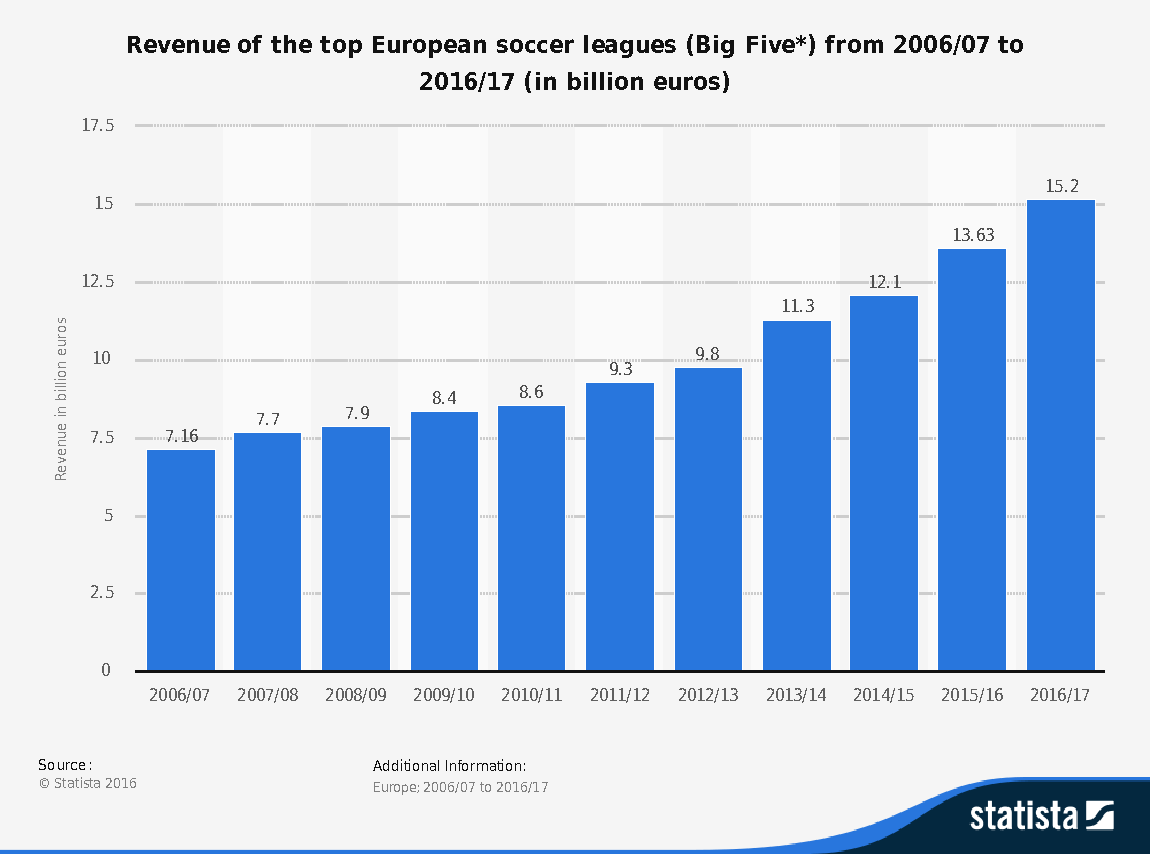
\includegraphics[width=1.0\textwidth]{Figure1}}
{Revenue of the top European soccer leagues (Big Five*) from 2006/07 to 2016/17 (in billion euros)\label{Fig1}}
{Notes}
\end{figure}

\begin{figure}
\FIGURE
{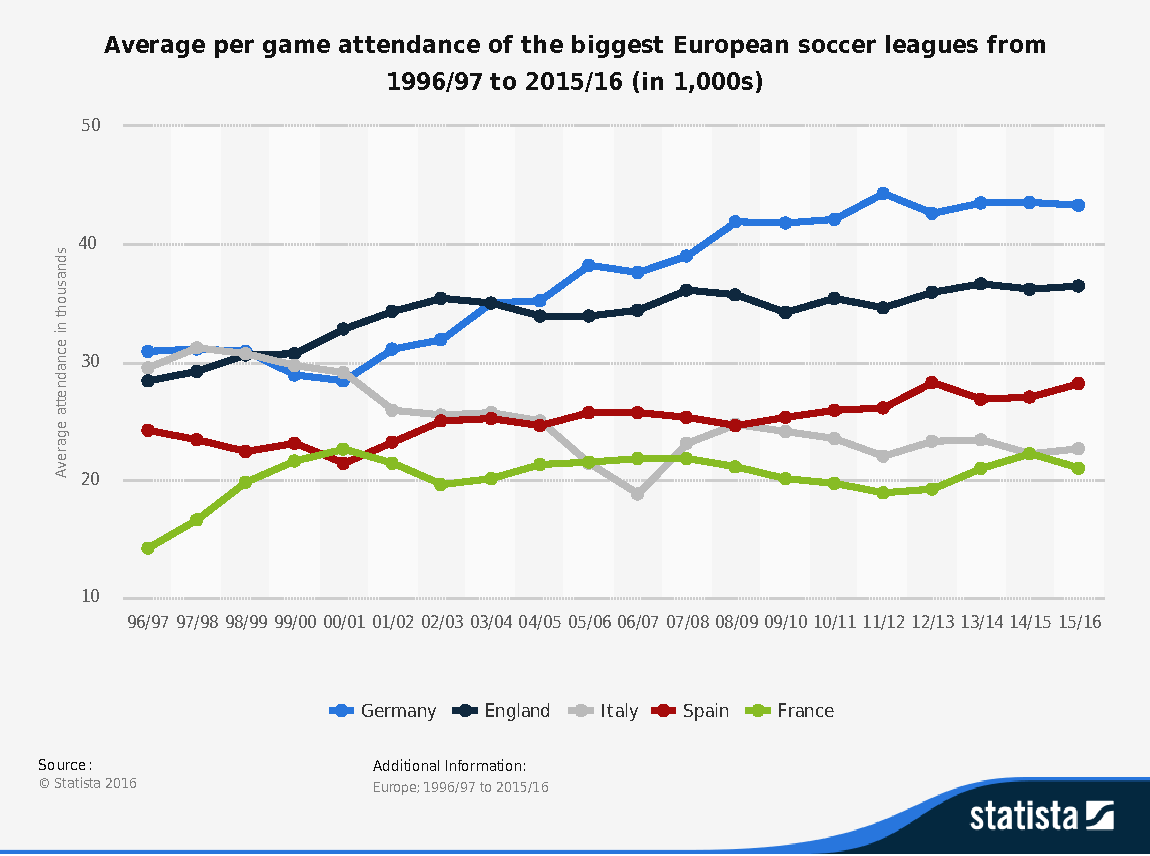
\includegraphics[width=1.0\textwidth]{Figure2}}
{Average per Game Attendance of the Biggest European Soccer Leagues from 96/97 t0 2015/16 (in thousands)\label{Fig2}}
{}
\end{figure}

\begin{figure}
\FIGURE
{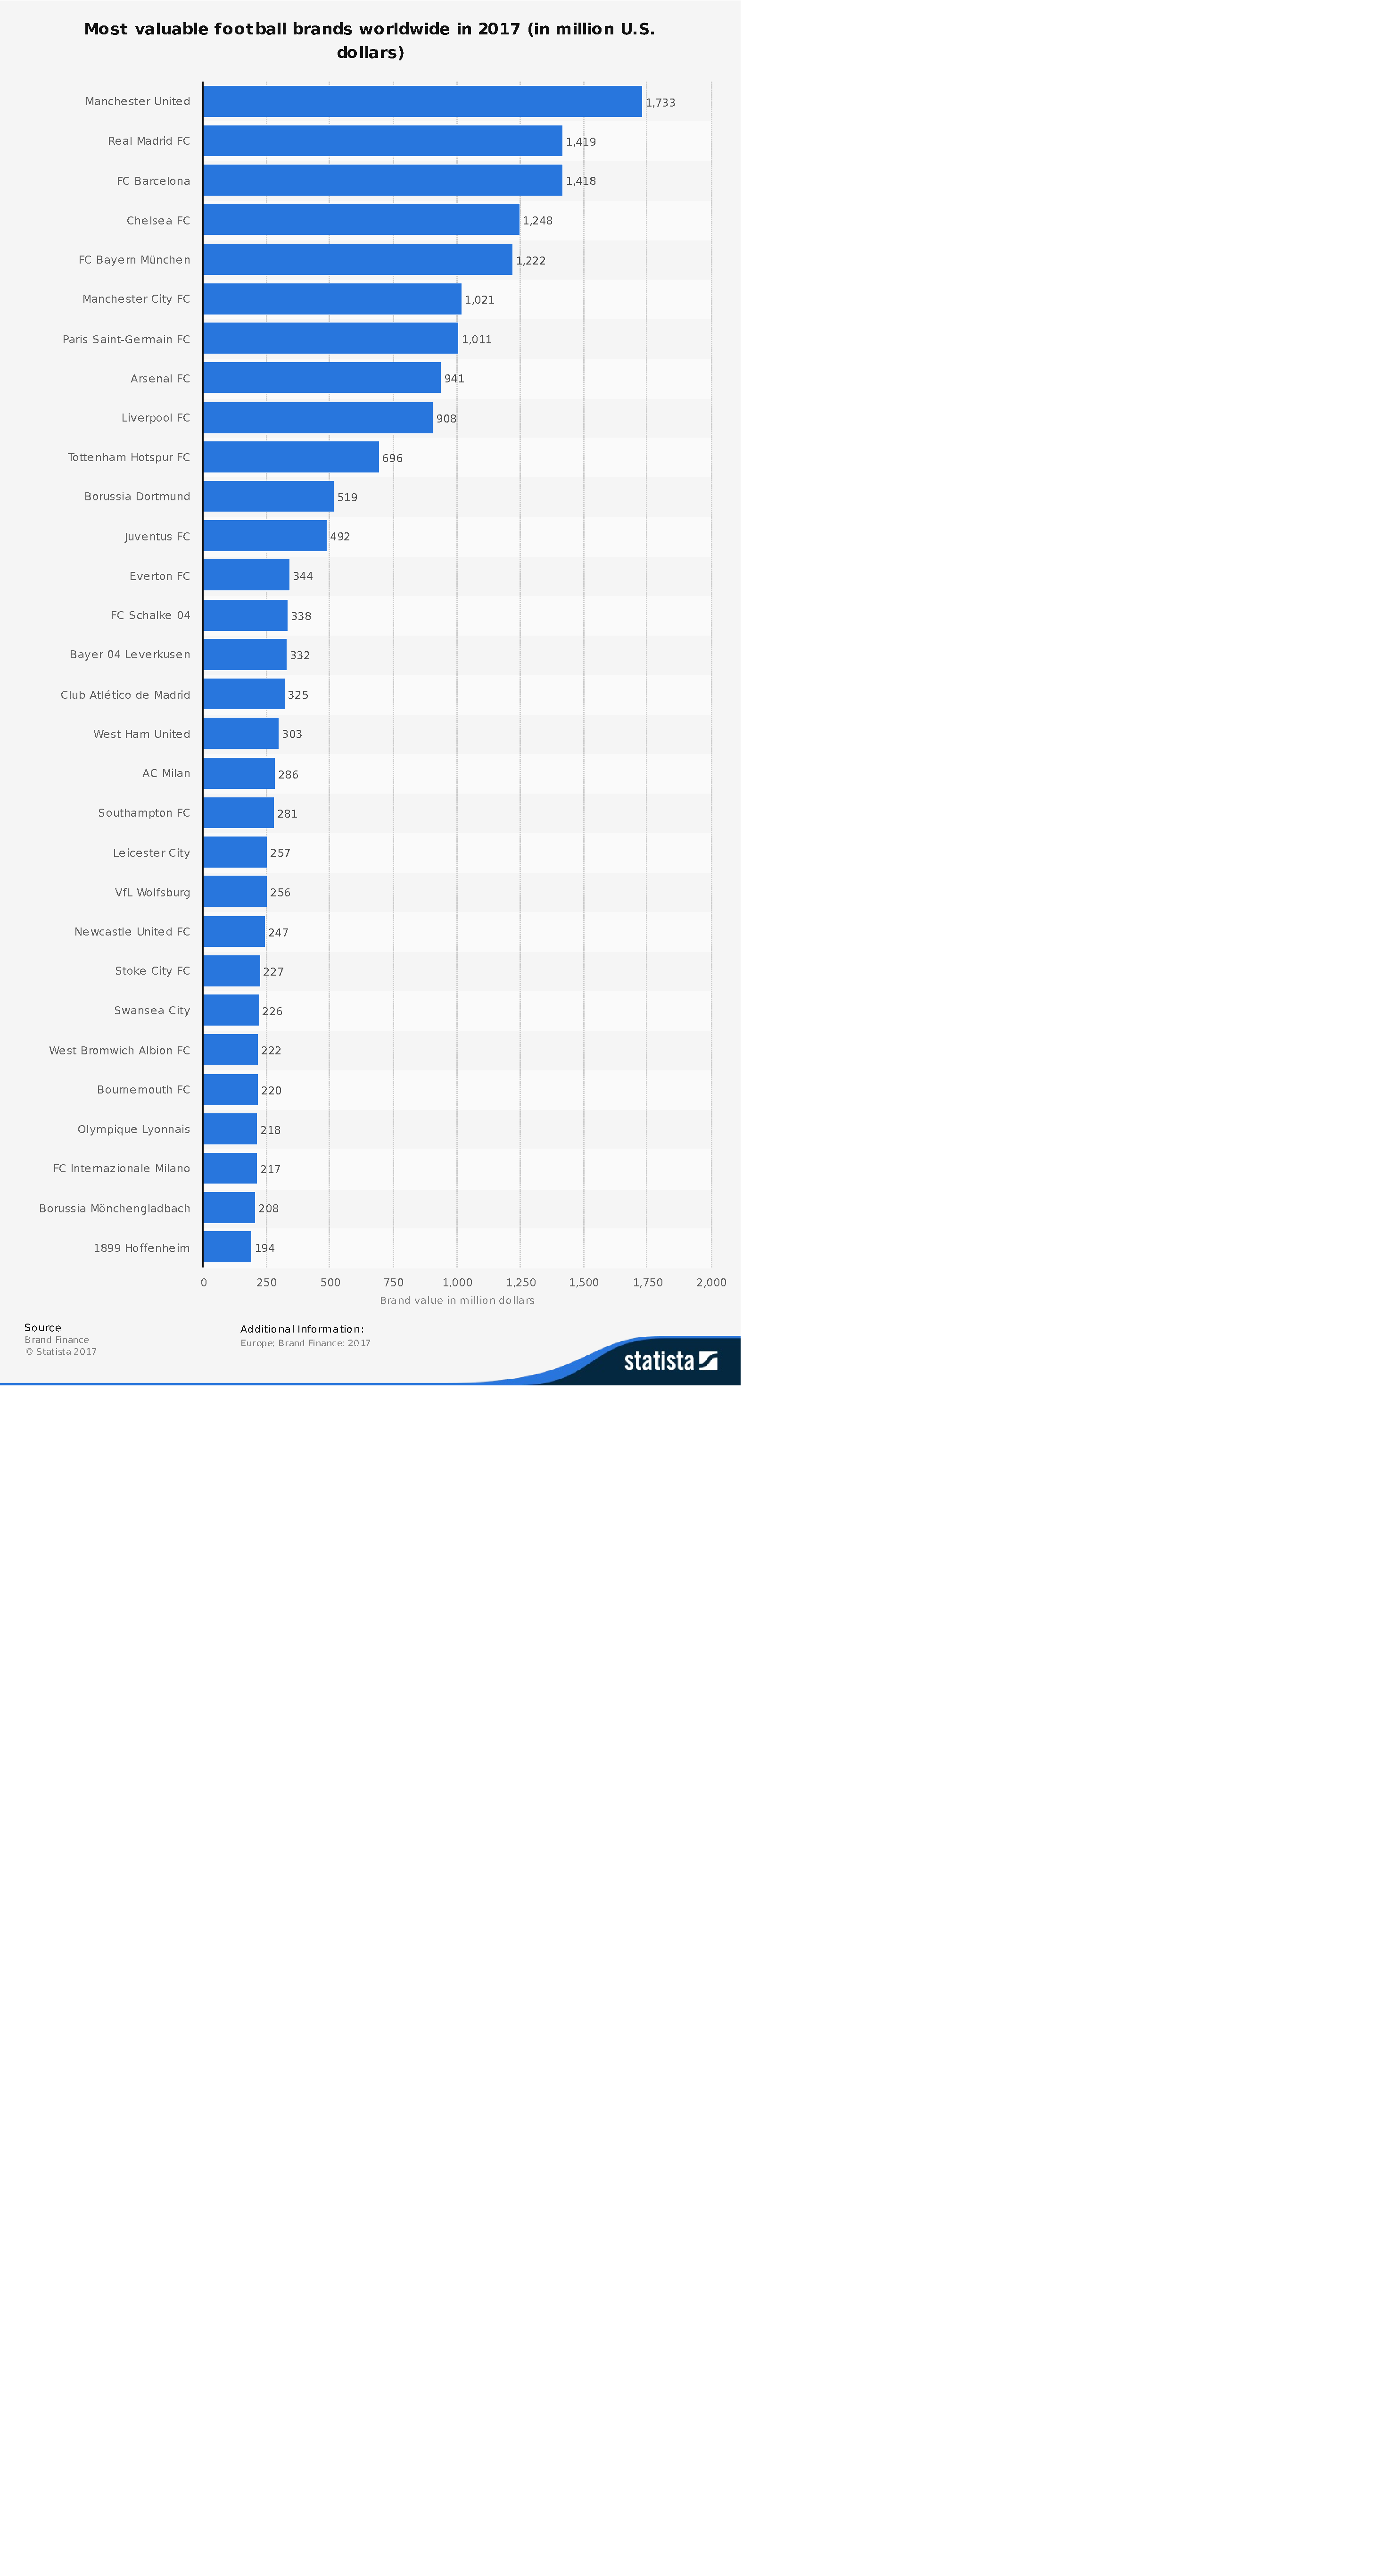
\includegraphics[height = 1.0\textheight, width = 1.0\textwidth]{Figure3}}
{Most Valuable Soccer Brands in 2017 (in million U.S. \$)\label{Fig3}}
{}
\end{figure}

\begin{figure}
\FIGURE
{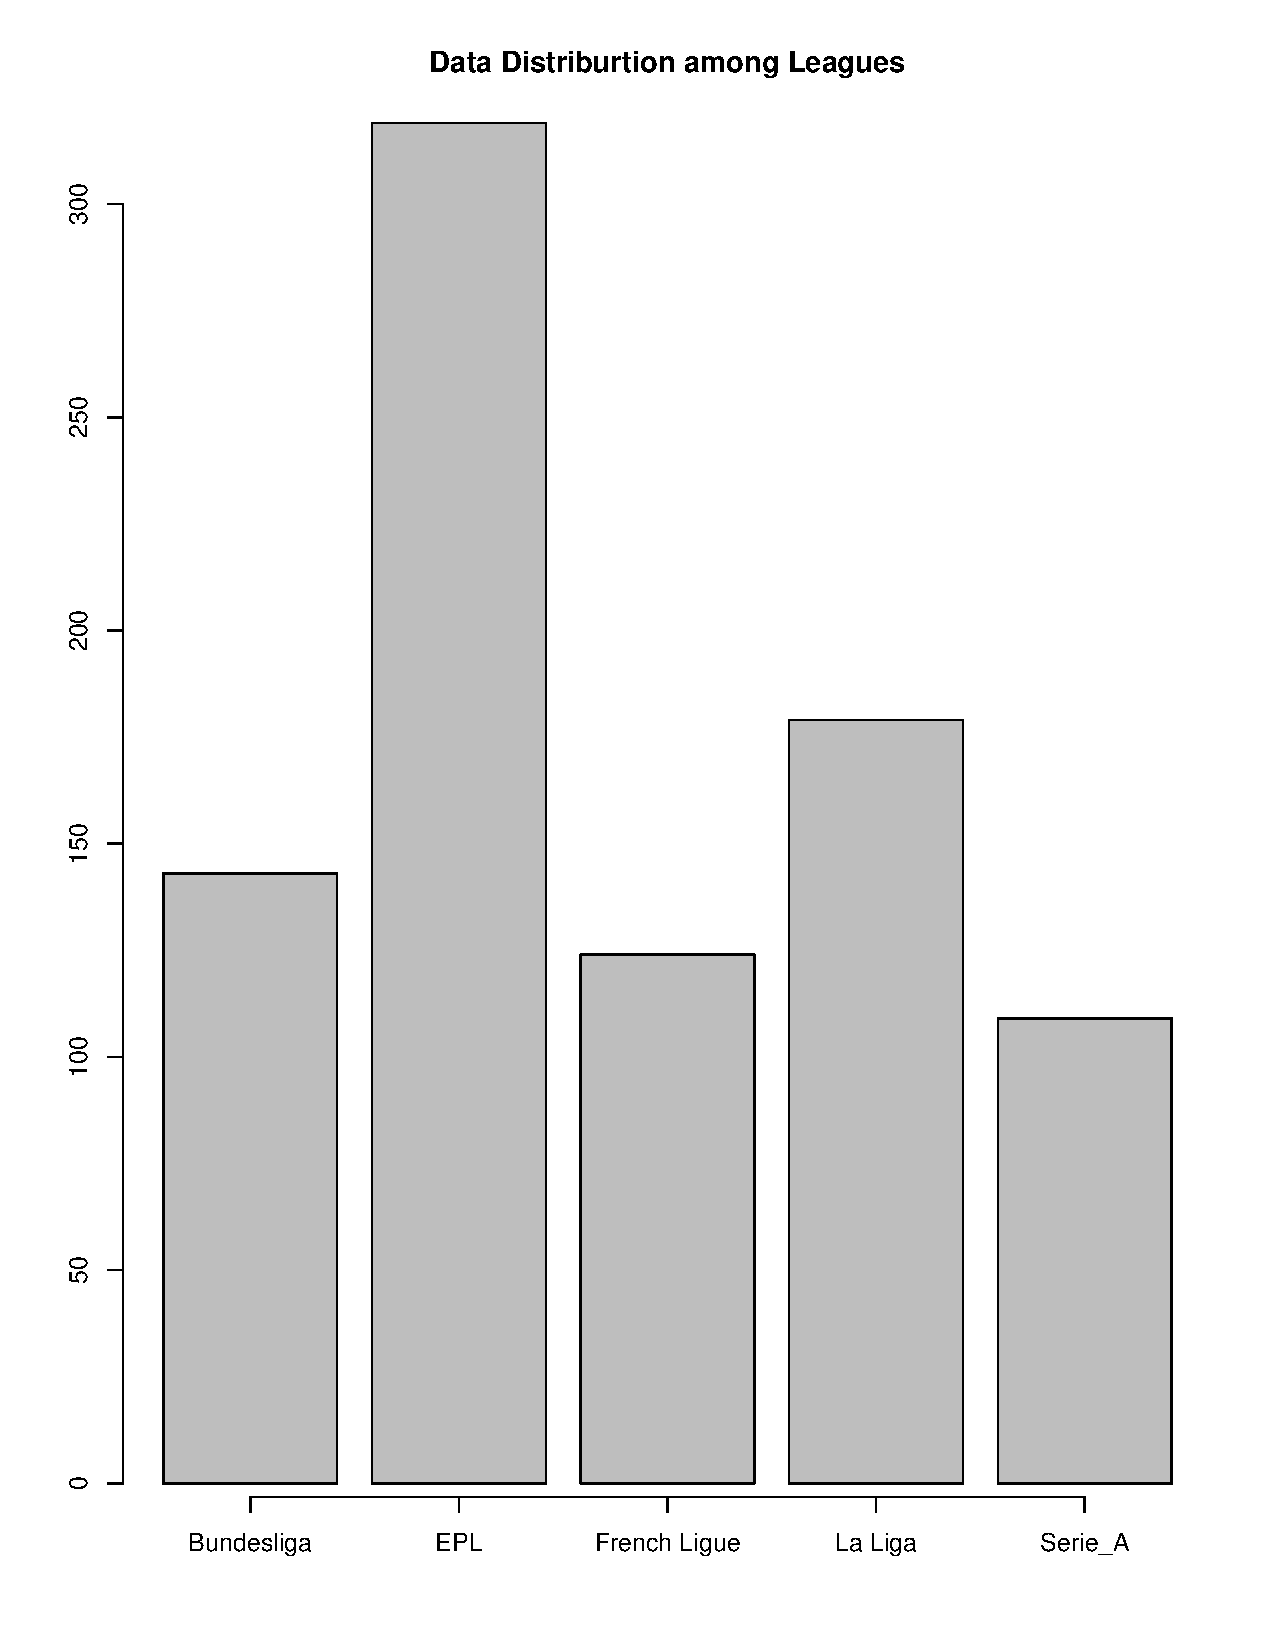
\includegraphics[height = 0.5\textheight, width = 0.6\textwidth]{Figure4}}
{Club-Seasons by League\label{Fig4}}
{}
\end{figure}

\begin{figure}
\FIGURE
{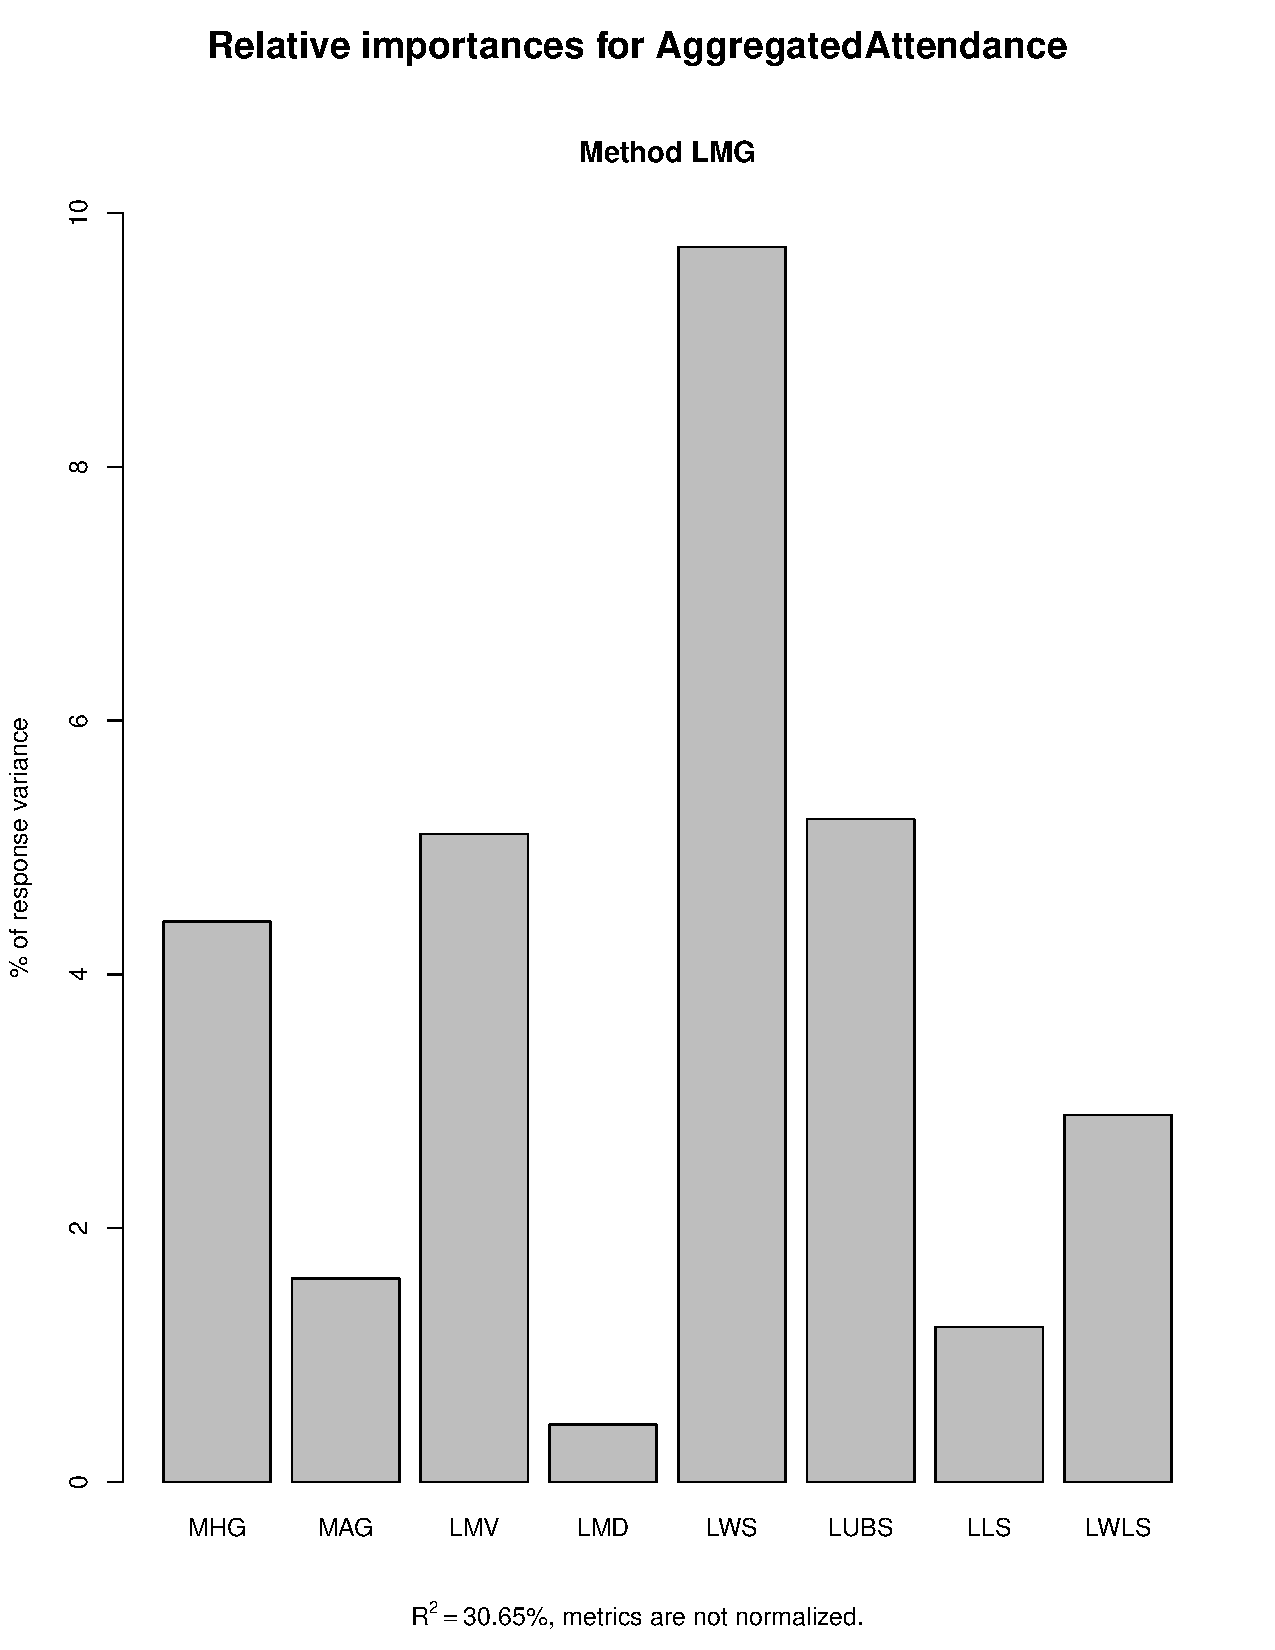
\includegraphics[height = 0.5\textheight, width = 0.6\textwidth]{Figure5}}
{Relative Importance by Team Performance Metrics\label{Rel}}
{}
\end{figure}

\begin{figure}
\FIGURE
{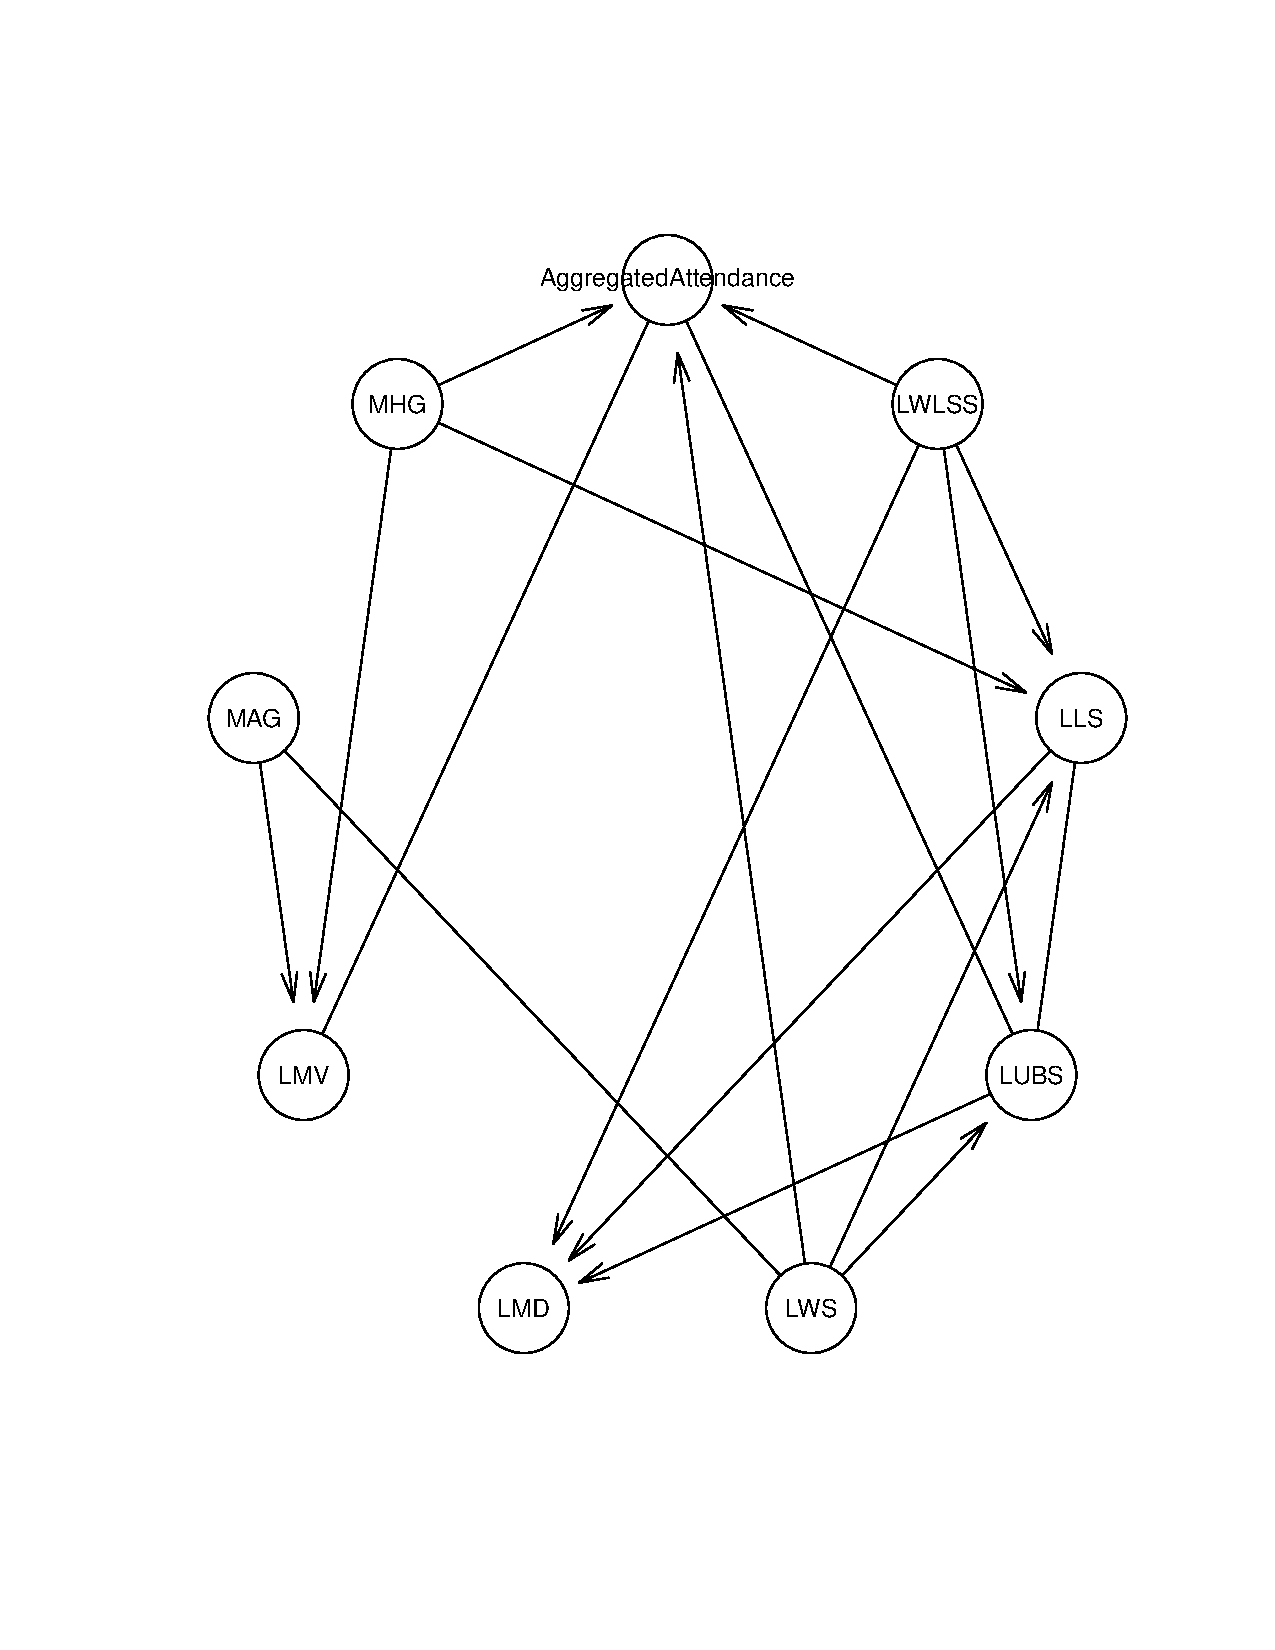
\includegraphics[height = 0.5\textheight, width = 0.6\textwidth]{Figure6}}
{Bayesian Network Graphical Model\label{Bayes}}
{}
\end{figure}
%=========================

% Appendix here
% Options are (1) APPENDIX (with or without general title) or 
%             (2) APPENDICES (if it has more than one unrelated sections)
% Outcomment the appropriate case if necessary
%
% \begin{APPENDIX}{<Title of the Appendix>}
% \end{APPENDIX}
%
%   or 
%
% \begin{APPENDICES}
% \section{<Title of Section A>}
% \section{<Title of Section B>}
% etc
% \end{APPENDICES}


% References here (outcomment the appropriate case) 

% CASE 1: BiBTeX used to constantly update the references 
%   (while the paper is being written).
%\bibliographystyle{informs2014} % outcomment this and next line in Case 1
%\bibliography{Soccer_Interfaces} % if more than one, comma separated

% CASE 2: BiBTeX used to generate mypaper.bbl (to be further fine tuned)
%\input{mypaper.bbl} % outcomment this line in Case 2

\end{document}


